\subsection{Context-aware Long-term Goal Prediction}

We propose to use a more sophisticated trajectory forecasting algorithm, that can make more realistic predictions, which in the end improve the overall result for the motion legibility.
%
We assume using a multi-modal prediction algorithm in Eq. (\ref{eq_dragan9}) that also takes into account the contextual cues $C$:

\begin{equation}
    \label{eq_P_G_with_context}
     P\left(G \mid \xi_{S \rightarrow \xi(t)}, C \right) 
\end{equation}

\noindent
Now, in order to improve the legibility of the robot motion, we can minimize the entropy of $G$:

\begin{equation}
    \label{eq_H_G}
    \min H(G) = -\mathbb{E} \left[\log P(G \mid \xi_{S \rightarrow \xi(t)}, C ) \right]
\end{equation}

We are inspired by the Inception Score in Generative Models literature, which propose to use a pre-trained neural network (the Inception Net [REF] trained on the
ImageNet [REF]) to ensure the generated samples are highly classifiable [REF]. Here, we are also interested in generating motions that are as classifiable as possible for the observers and in order to simulate the way an observer perceives and interpret the surrounding trajectories, we propose to use an independent prediction model that is trained on a dataset of motion trajectories.
We will discuss the potential bias of the proposed method in the Conclusion section [REF].

We decided to use the GoalGAN architecture [REF] to estimate \ref{eq_P_G_with_context}, which is trained on a relatively large dataset of long-term human trajectories. The model is in fact proposed to first estimate the goals.


\subsection{Using LLMs to Describe Potential Goals:}

Query: 



\begin{figure}[ht]
  \centering
  \begin{subfigure}{0.8\textwidth}
    \textbf{Query:} Given the robot's task of delivering dishes, along with the image and the characteristics of the environment, what could be the potential positions that the robot aims to reach?
    \vspace{10pt}
  \end{subfigure}

  \begin{subfigure}{\textwidth}
  \centering
    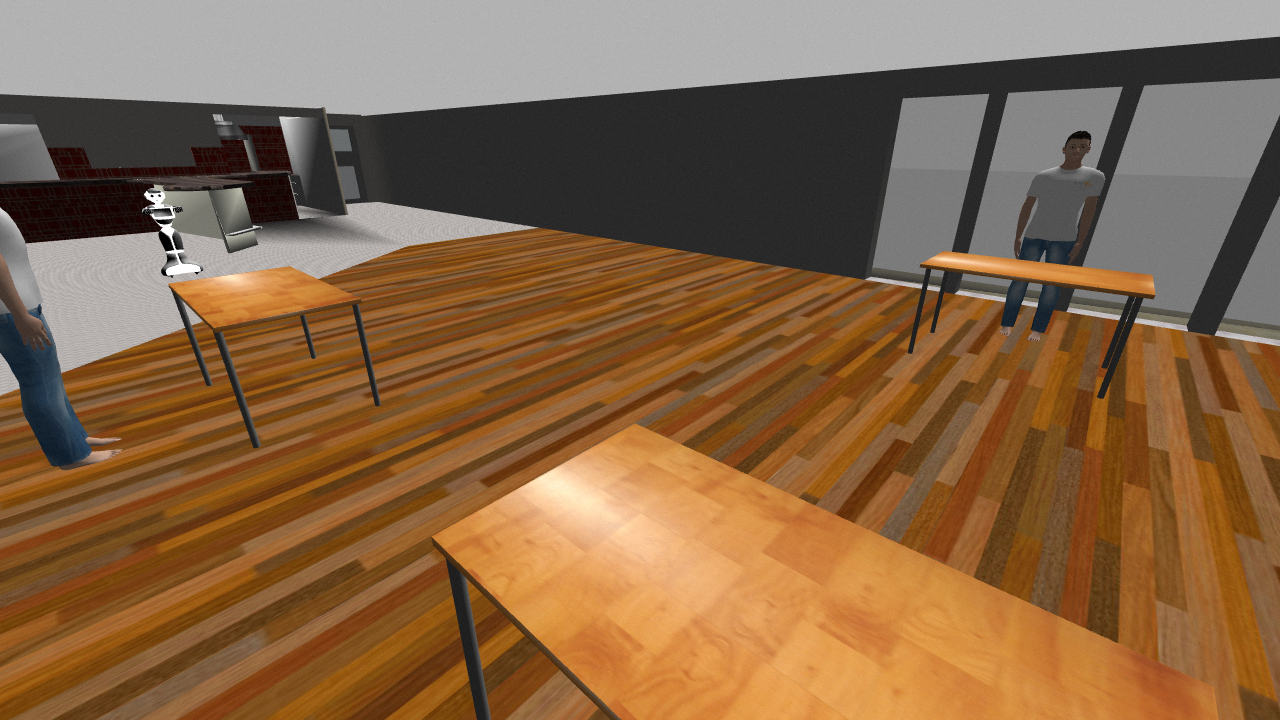
\includegraphics[width=0.8\linewidth]{figs/pepper-in-restaurant.png}
    \caption{Pepper Working in a Restaurant}
  \end{subfigure}

  \begin{subfigure}{\textwidth}
    \vspace{10pt}
    \textbf{Answer:} 
        The robot's potential goal positions for delivering dishes in the provided image are near the tables. Multiple tables around the room could serve as delivery points. Specifically: \\
        - The table closest to the robot and in front of the person wearing blue jeans could be a goal position. \\
        - The table on the far left, near the person standing by the window, is another potential goal position. \\
        - Any other visible tables in the room could also serve as goal positions based on the robot's needs.
  \end{subfigure}

  \caption{Asking AGI for Potential Goals of the Robot}
  \label{fig:vqa_example}
\end{figure}


\subsection{Synthesizing Legible Motions}
We need to modify the planner to become legibility-aware. This can happen by adding a gradient-descent-based process that iteratively updates the initial proposed trajectory to reach to the desired legibility score:


% \begin{figure}
%     \centering
%     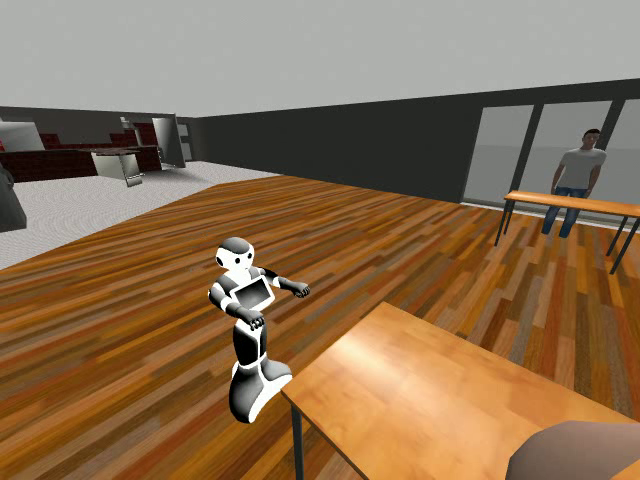
\includegraphics[width=0.6\textwidth]{figs/legibot-pepper-restaurant.png}

%     \caption{GoalGAN}
%     \label{fig:enter-label}
% \end{figure}


